% Master-Konferenzseminar, FH Suedwestfalen
%
% Vorlage ist xelatex-kompatibel
% Literatur in seminar.bib
% Build-Prozess:
%  xelatex seminar; bibtex seminar; xelatex seminar; xelatex seminar
%
%
\documentclass[twoside,a4paper]{IEEEtran}
\usepackage{fontspec}
\usepackage[ngerman]{babel}
\usepackage{cite}
\usepackage{xcolor}
\usepackage{listings}
\usepackage{graphicx}
\usepackage{multicol}
\lstset{basicstyle=\footnotesize\ttfamily,breaklines=true}
\lstset{numberstyle=\tiny\color{blue},keywordstyle=\color{blue}}
\usepackage{blindtext}  % <-- kann weg!
% Custom
\renewcommand{\thepage}{X-\arabic{page}}
\begin{document}
% paper title
% can use linebreaks \\ within to get better formatting as desired
\title{Erkennung japanischer Schriftzeichen \\mittels maschinellen Lernens%
    \thanks{%
    Dieser Beitrag entstand im 
    Rahmen des Master"=Konferenzseminars \emph{info@swf 2022}, das im
    Wintersemester 2021/22 vom Fachbereich Informatik und
    Naturwissenschaften der Fachhochschule Südwestfalen
    durchgeführt wurde.}}
% author names and affiliations
% use a multiple column layout for up to three different
% affiliations
\author{
  \IEEEauthorblockN{N.N.\\ }
  \IEEEauthorblockA{Fachhochschule Südwestfalen}
}

\maketitle


%%% Zusammenfassung
\begin{abstract}
Das japanische Schriftsystem ist mit drei verschiedenen Alphabeten (Hiragana, Katakana, Kanji) eines der komplexesten Schriftsysteme der Welt. Eine Person muss dabei ca. 2000 Schriftzeichen erlernen, um eine Zeitung vollständig verstehen zu können. In dem Paper „Recognizing Handwritten Japanese Characters Using Deep Convolutional Neural Networks” von Charlie Tsai wurde eine Erkennung mittels der VGGNet, speziellen Architekturen Konvolutionaler Neuronaler Netze, erprobt. Im Ansatz wurde dabei sowohl die separate Erkennung aller Alphabete als auch die gemeinsame aller möglichen Schriftzeichen erforscht. Dabei konnten Testgenauigkeiten von bis zu 99,53\% erreicht werden. In diesem Paper sollen die Ergebnisse nachvollzogen und mit weiteren Mitteln die Qualität des Modells überprüft werden. Dies soll den Einsatz und Vergleich weiterer Netzwerkarchitekturen wie beispielsweise der Vision Transformer oder ResNet ermöglichen. Zusätzlich wurden weitere moderne VGG und ResNet Architekturen gesichtet und mit dem implementierten Mitteln überprüft. Auch ein Einsatz weiterer Datensätze aus der vorliegenden Datenbank wurde erprobt. 
\end{abstract}


%%% Text beginnt
\section{Einleitung}
Die japanische Sprache ist eine der komplexesten Sprachen der Welt. Besonders für Muttersprachler europäischer Sprache sind die hohen Abweichungen in Aussprache, Grammatik und Schriftsystem ein Grund für große Probleme beim Erlernen der Sprache. Laut dem FSI ist Japanisch, neben Sprachen wie Arabisch, Koreanisch und Chinesisch, eine Kategory IV Sprache, welche mindestens 2200 Lernstunden für englische Muttersprachler benötigen und damit als eine der schwierigsten Sprachen der Welt gilt \cite{FSI}.

Geteilt in drei Alphabete (Hiragana, Katakana, Kanji) muss ein Schüler des Japanischen über 2000 Schriftzeichen erlernen, um eine Zeitung ohne Hilfe lesen zu können. Dazu kommt zusätzlich im Falle der Kanji nicht nur die Bedeutung sondern auch verschiedene Lesungen, welche von einigen bis in Dutzende pro Zeichen reichen können \cite{ABOUT_JAPANESE}.

Schüler des Japanischen können heutzutage auf viele Tools zurückgreifen, um ihren Lernvorgang zu unterstützen. Auch gibt es einige Apps, welche die automatische Erkennung von japanischen Schriftzeichen ermöglichen. In Charlie Tsais Paper "Recognizing Handwritten Japanese Characters Using Deep Convolutional Neural Networks" konnte dieser bis zu 99,53\% aller Schriftzeichen der ETL Character Database, einer Datenbank von handgeschriebenen japanischen Schriftzeichen, korrekt klassifizieren \cite{RHC}. Diese Ergebnisse sollen in diesem Projekt durch den Einsatz der genutzten VGGNet nachvollzogen und falls möglich durch die Nutzung weiterer Techniken wie Vision Transformer oder ResNet verbessert werden. Dazu wird zunächst auf die Grundlagen dieser Arbeit eingegangen, um im Folgenden die eingesetzten Daten darzustellen. Danach können verschiedene Modelle für das maschinelle Lernen aufgestellt und deren Ergebnisse vorgestellt werden. Schließlich wird ein Fazit und ein Ausblick auf mögliche nächste Arbeiten gegeben.

Für den praktischen Teil der Arbeit wurde Python 3 mit Keras und Tensorflow 2 verwendet.
\section{Grundlagen}
Im folgenden Abschnitt sollen kurz die Grundlagen der eingesetzten Modelle dargestellt werden. Dabei wird zunächst auf die Konvolutionale Neuronale Netze und dann auf die Vision Transformer eingegangen. Grundlagen zu Neuronalen Netzen werden dabei als gegeben angesehen.
\subsection{Konvolutionale Neuronale Netze} %11.11
Konvolutionale Neuronale Netze oder Convolutional Neural Networks sind Neurale Netze, die vom visuellen Cortex des Gehirns inspiriert wurden. Hierbei sind Neuronen in unteren Schichten für die Erkennung primitiver Formen verantwortlich, während Neuronen in höheren Schichten auf immer komplexere Muster reagieren \cite[S.360]{MACHINE_LEARNING}. 
\begin{figure}[!htb]
	% \centering
	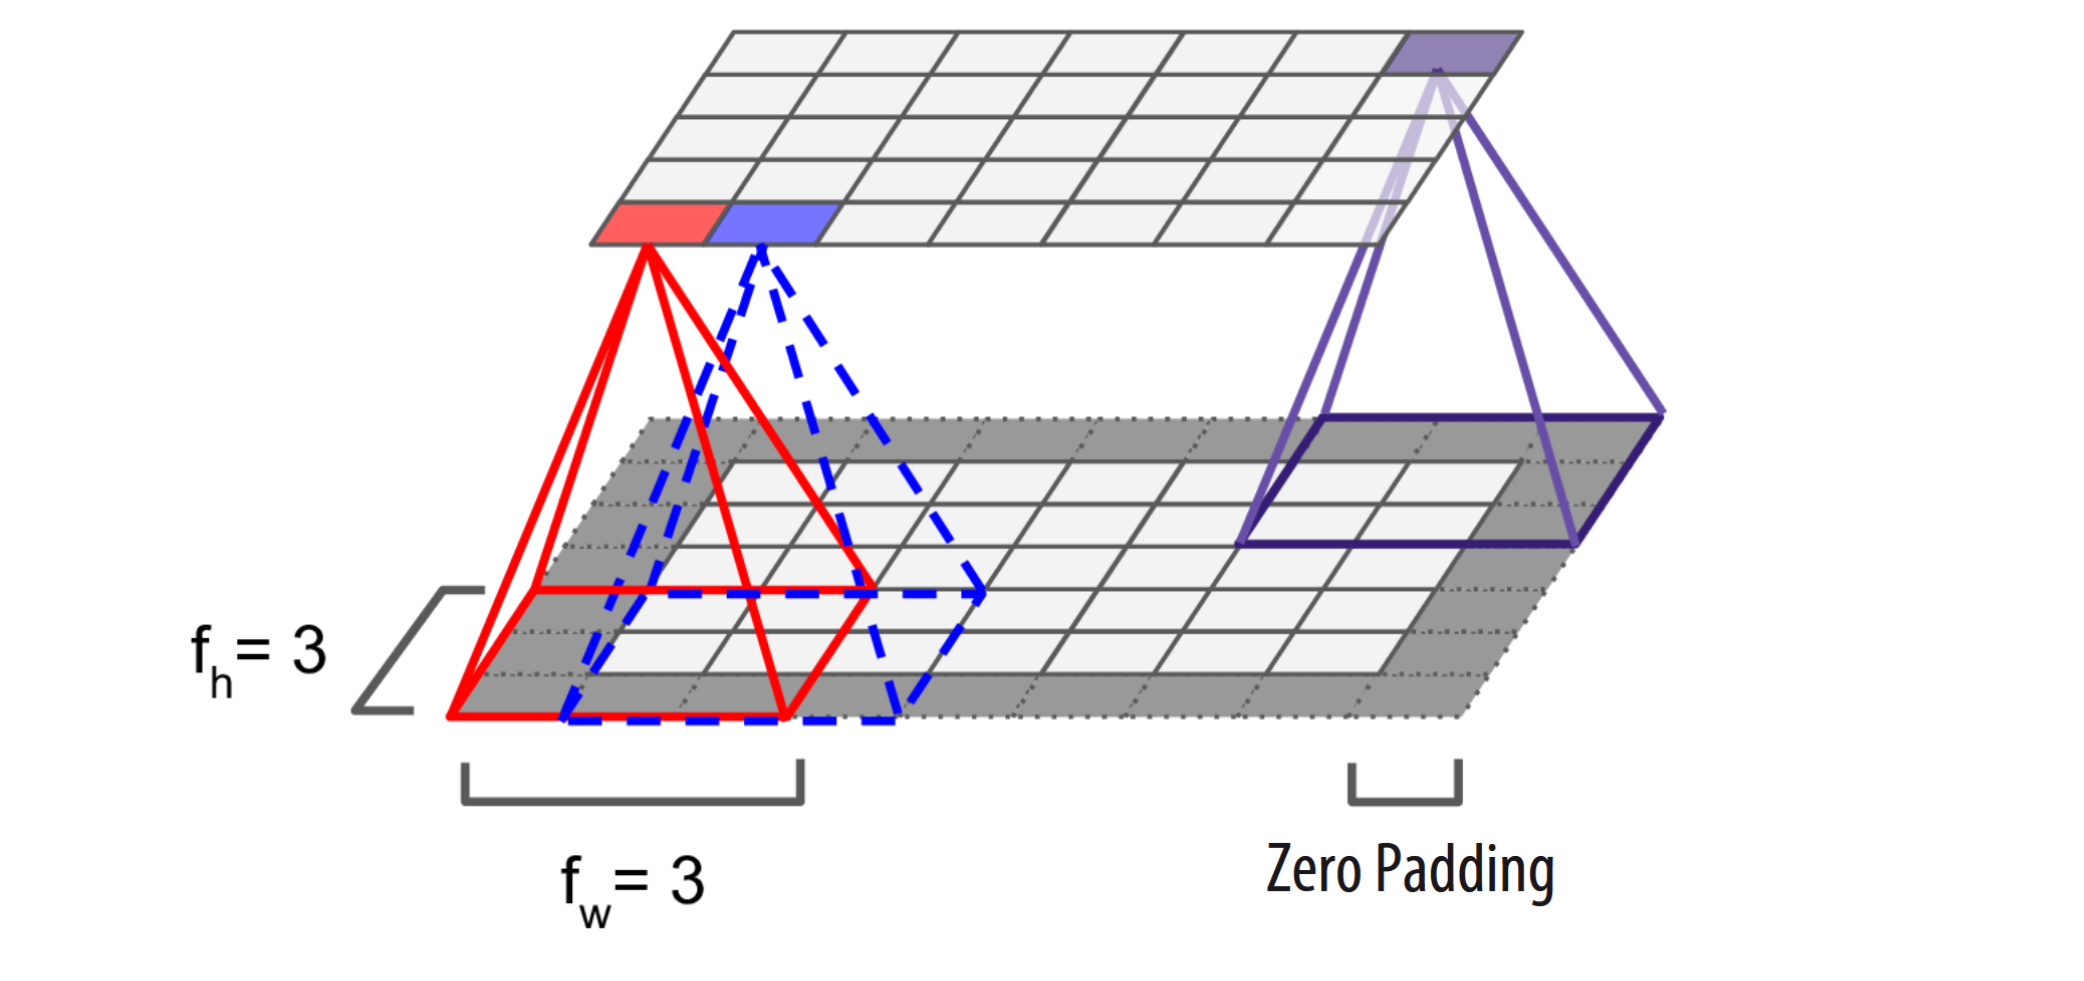
\includegraphics[width=\columnwidth]{cnn}
	\caption{Aufbau einer konvolutionalen Schicht mit Schrittweite eins und Zero Padding \cite[S.362]{MACHINE_LEARNING}.}
	\label{bild1}
\end{figure}

In der Praxis haben sich hier sogenannten konvolutionale Schichten mit einem bestimmten Wahrnehmungsfeld mehrere Pixel etabliert, welche  ihre Eingabe mit einer Schrittweite (Stride) analysieren und so aus den Pixeln eine neue Ausgabe erzeugen \cite[S.361-363]{MACHINE_LEARNING}. Diese Eingaben können beispielsweise Bilder oder Ausgaben vorherigen konvolutionaler Schichten sein. Die Ränder der aktuellen Eingabe werden dabei in der Regel mit einem Padding, einem Randbereich bestimmter Zahlen um die originale Eingabe, versehen, um eine kleiner werdende Ausgabe zu verhindern, falls dies nicht gewünscht ist \cite[S.361-363]{MACHINE_LEARNING}. Die Eingabe des Wahrnehmungsfelds wird mittels eines sogenannten Filters gewichtet, bevor ein Ausgabepixel erzeugt wird. Filter lassen sich als kleine Bilder visualisieren, welche auf bestimmte Formen in der Ausgangsschicht reagieren \cite[S.363]{MACHINE_LEARNING}. 

\begin{figure}[!htb]
	% \centering
	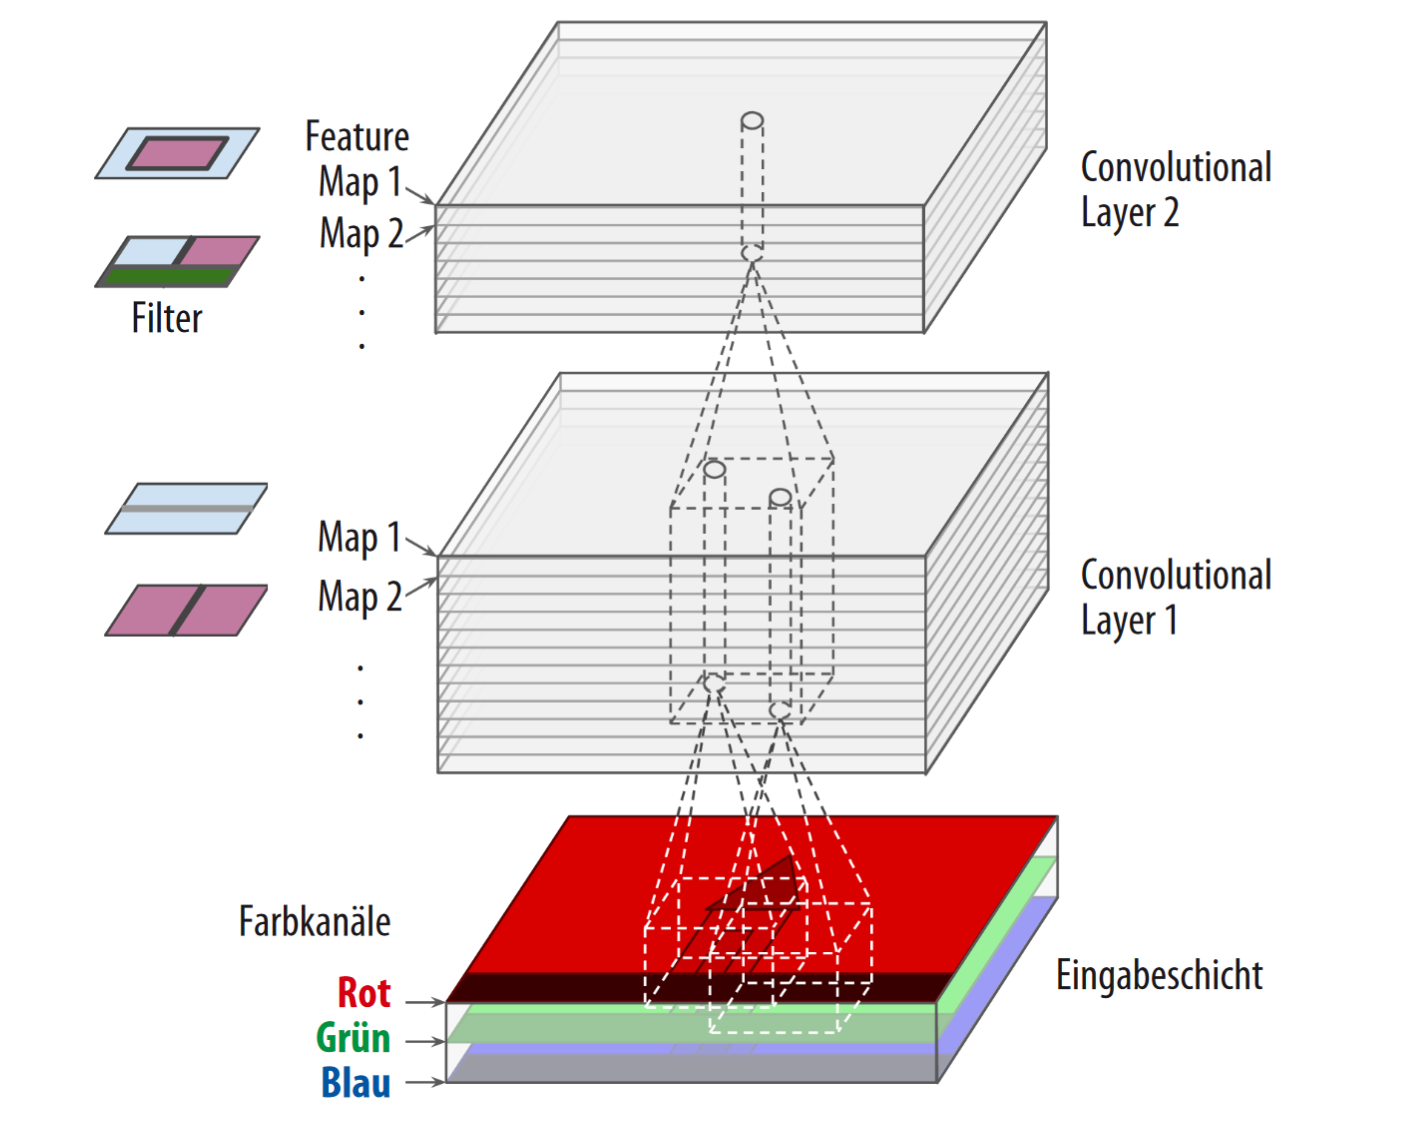
\includegraphics[width=\columnwidth]{cnn_example}
	\caption{Aufbau eines CNN mit drei Schichten und vielen Feature Maps \cite[S.365]{MACHINE_LEARNING}.}
	\label{bild1}
\end{figure}

Pro konvolutionaler Schicht können nun mehrere Filter, sogenannte Feature Maps, auftreten, welche die Erkennung verschiedener Formen in der vorherigen Schicht erlauben und in tieferen Schichten die Kombination vorheriger Features ermöglichen. Tatsächlich erstreckt sich nun das Wahrnehmungsfeld über alle vorherigen Feature Maps, was in einer dreidimensionalen Gewichtsmatrix resultiert \cite[S.364-365]{MACHINE_LEARNING}. Diese Art des Vorgehen erlaubt zusätzlich eine Analyse von Farbbildern mit mehreren Kanälen. Typischerweise wird durch eine passende Wahl von Strides und Filtern eine Komprimierung der Bildgröße bei Steigerung der Feature Maps angestrebt. Eine Komprimierung kann dabei aber nicht nur durch Strides, sondern auch durch Pooling Layer geschehen. Ein Pooling Layer betrachtet in der Regel einen gewissen zweidimensionalen Bereich einer Ausgabe und komprimiert diesen auf eine vom Typ des Layers abhängige Weise. Hierdurch entsteht eine Komprimierung der Ausgabe der vorherigen konvolutionalen Schicht. Eine typische Art von Pooling ist das Max-Pooling, bei welcher die größte Zahl des betrachteten Bereichs übernommen wird \cite[S.369-370]{MACHINE_LEARNING}. In den meisten Architekturen von CNNs, wird am Ende die Ausgabe der letzten konvolutionalen Schicht geebnet und mit einem Feed-Forward-Netz, die typische Variante Neuronaler Netze mit Schichten von Neuronen \cite[S.263]{MACHINE_LEARNING}, verbunden, welches dann Aufgaben wie Klassifikation vornehmen kann \cite[S.371]{MACHINE_LEARNING}. Einige verbreitete Architekturen von CNNs, welche auch in diesem Projekt erprobt wurden, sind das ResNet und VGGNet \cite[S.378-381]{MACHINE_LEARNING}.

\subsection{Vision Transformer} %12.11

Vision Transformer sind eine neue Technik des Maschinellen Lernens auf Basis der Transformer. Diese basieren vom Hauptprinzip auf einer sogenannten Attention und werden vorwiegend im Natural Language Processing eingesetzt, in welchem sie die vorher prävalenten Rekurrenten Neuronalen Netze weitgehend ablösen konnten \cite{TRANSFORMERS}. Wurden diese in Encoder-Decoder Netzen, spezielle Neuronale Netze bei welchen aus einer Eingabesequenz eine Ausgabesequenz erzeugt wird \cite[S.388-389]{MACHINE_LEARNING}, eingesetzt, so wurde bis zur Nutzung von Attentions nur ein letzter Zustand des Encoders als Eingabe im Decoder genutzt. Dies hat sich nach aktueller Forschung als Bottleneck herausgestellt, welches Rekurrenten Neuronale Netze besonders bei längeren Sätzen stark behindert hat \cite[S.2]{TRANSFORMERS}. Stattdessen wurden neue RNNs entworfen, welche es dem Decoder über eine erlernbare Attention erlauben sich in jedem Schritt auf andere Aspekte aller Zustände des Encoders zu konzentrieren \cite[S.4]{RNN_ATTENTION}.  

\begin{figure}[!htb]
	% \centering
	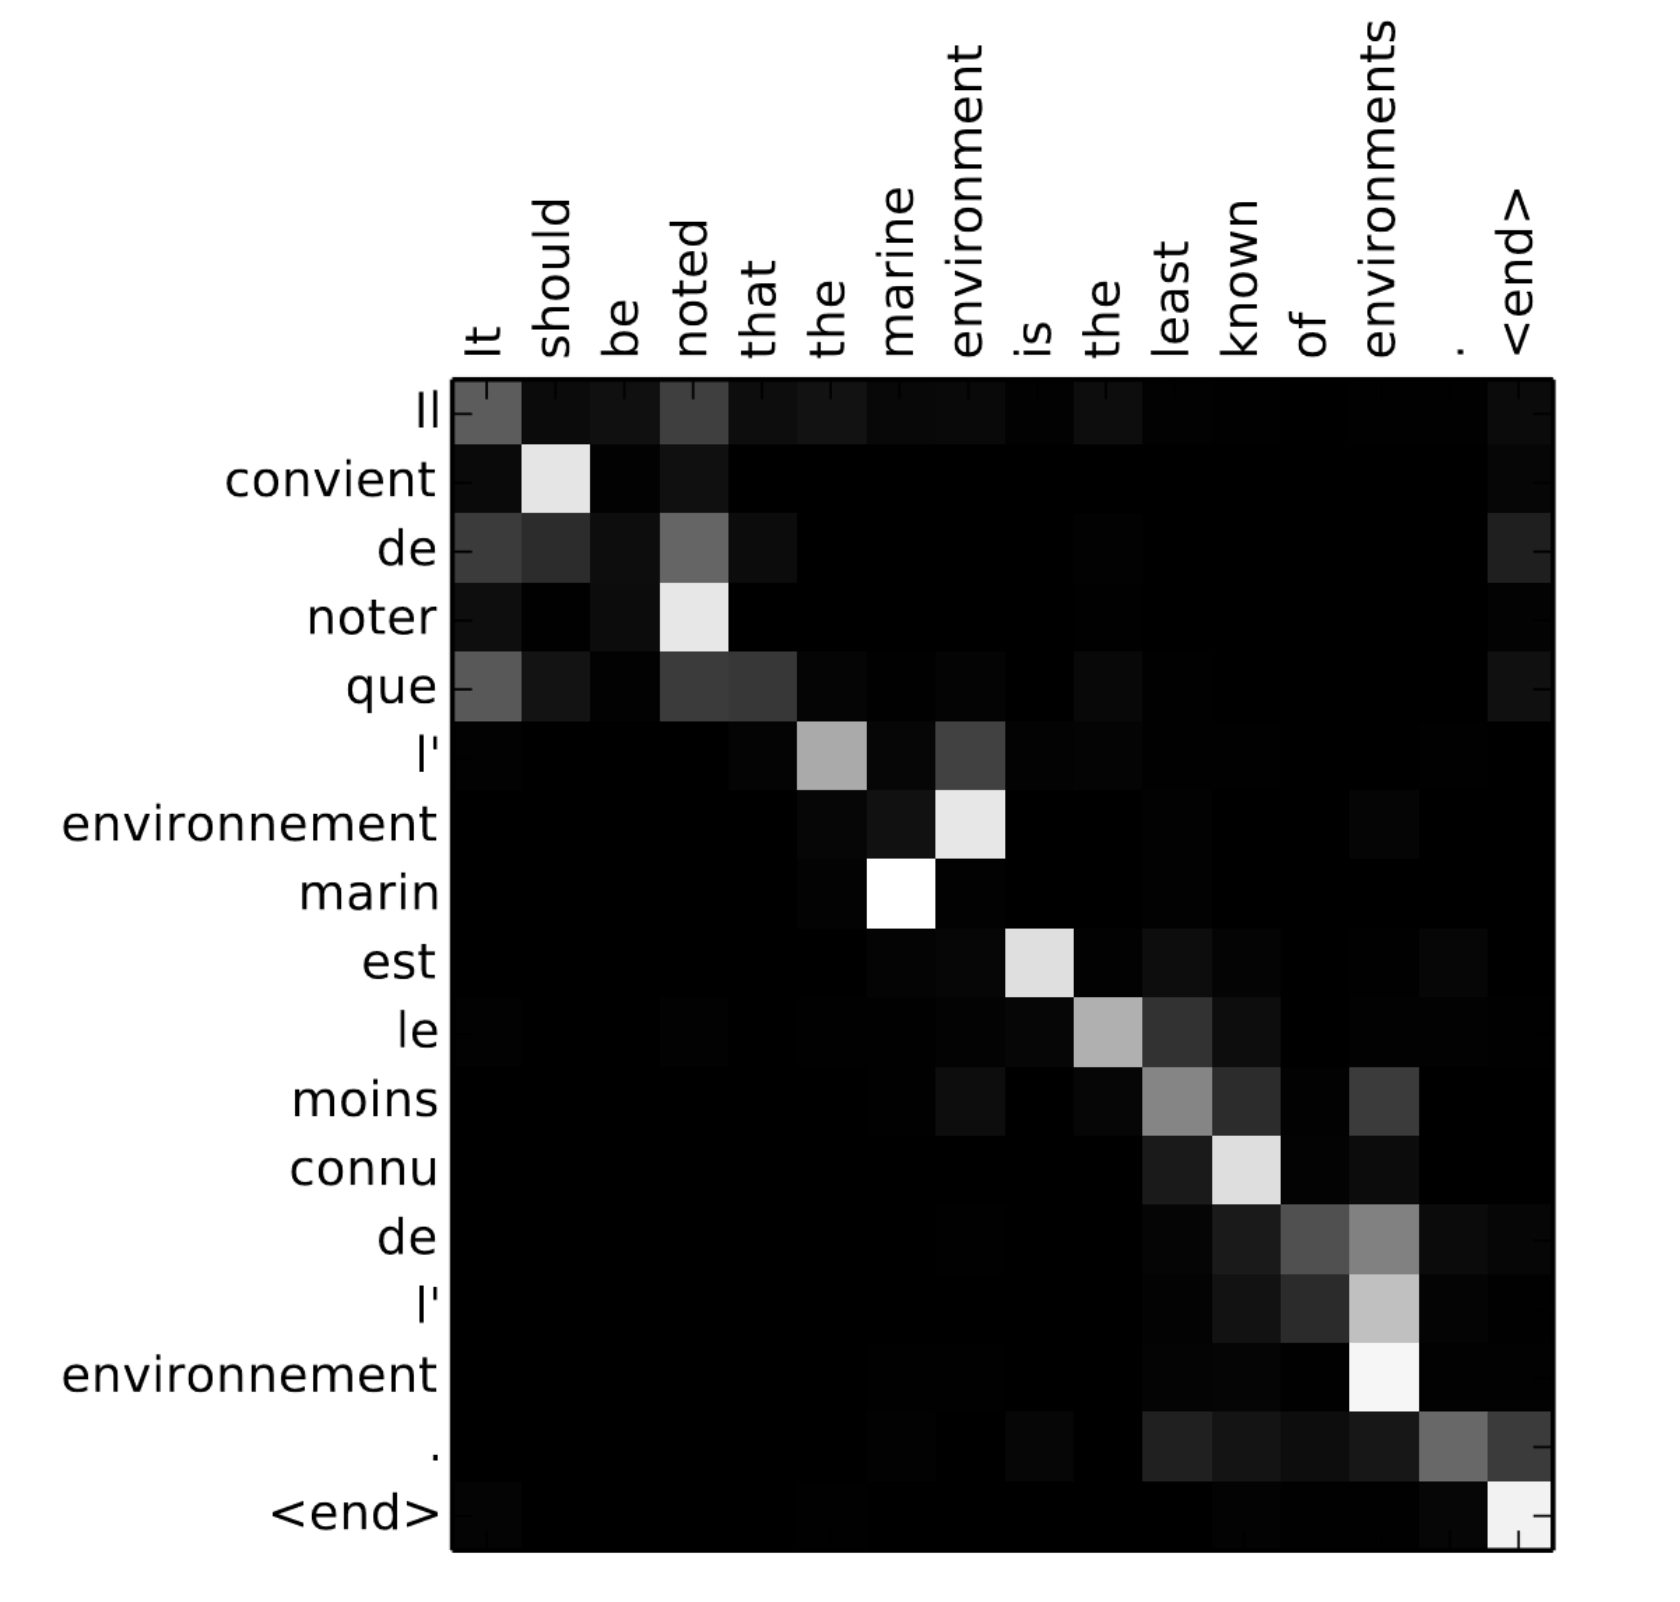
\includegraphics[width=\columnwidth]{attention_visualized}
	\caption{Beispiel für erlernte Attention zwischen einem englischen und französischen Satz \cite[S.6]{RNN_ATTENTION}.}
	\label{bild1}
\end{figure}
In weiteren Forschungen im Natural Language Processing hat sich herausgestellt, dass reine Netzwerke basierend auf Attention, also weiter oben genannten Transformer, RNNs als State of the Art können \cite[S.2]{TRANSFORMERS}. 

Vision Transformer sind vom Aufbau den Transformern im Natural Language Processing sehr ähnlich, besitzen jedoch im Fall von Klassifikation nur den Encoder der Transformer Modelle. Der grundsätzliche Aufbau lässt sich in der Abbildung \ref{vitimg} erkennen.

\begin{figure}[!htb]
	% \centering
	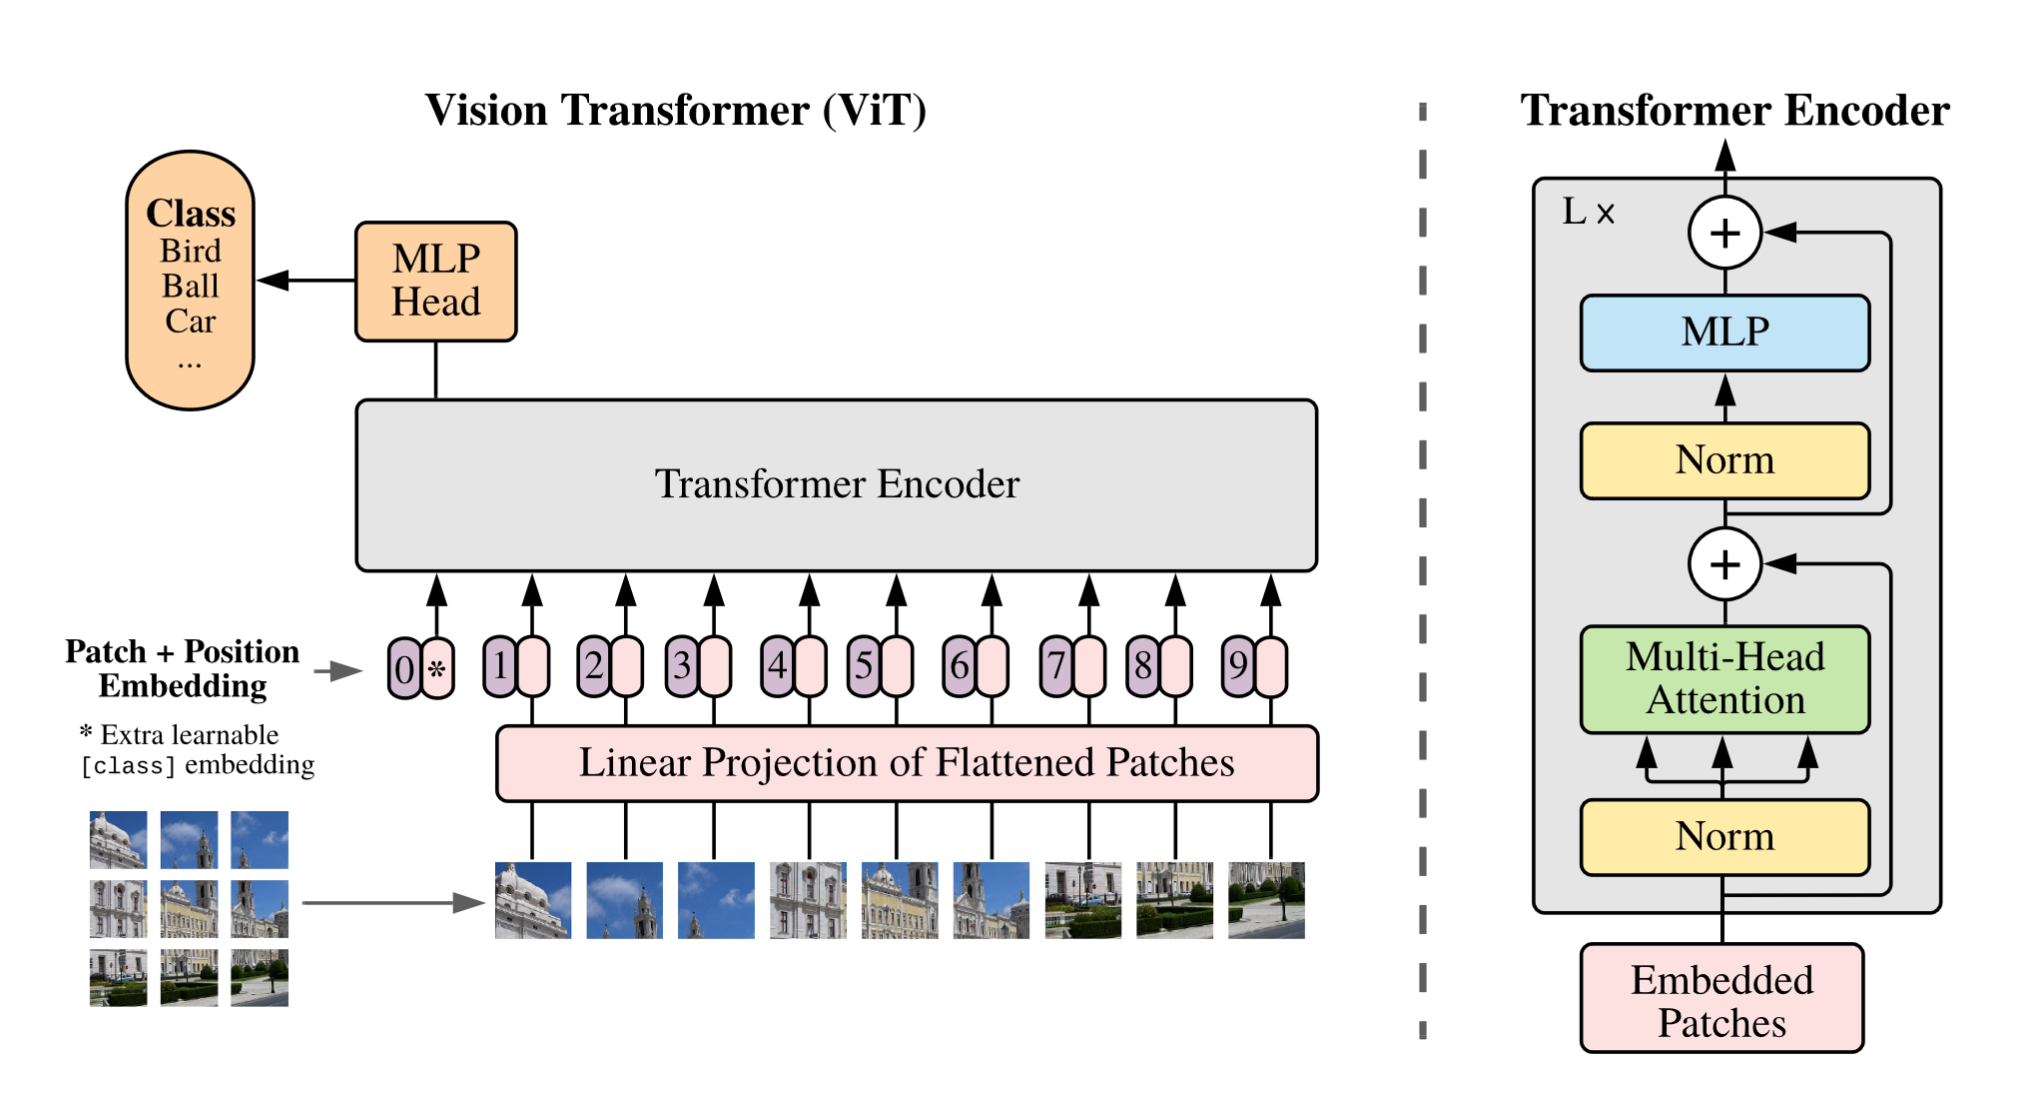
\includegraphics[width=\columnwidth]{vitimg}
	\caption{Grundsätzlicher Aufbau eines Vision Transformers \cite[S.3]{VIT}.}
	\label{vitimg}
\end{figure}

Dabei werden zunächst die Eingabebilder in mehrere zweidimensionale Bereiche einer vordefinierbaren Größe unterteilt, wobei ähnlich wie bei den CNNs ein Stride zum Überlappen von Bildbereichen genutzt werden kann. Danach werden die Eingabedaten über eine trainierbare lineare Projektion auf D, eine konstante vordefinierte Vektorgröße in allen Schichten des Transformers, Dimensionen reduziert und damit die sogenannten Patch-Embeddings generiert. Schließlich werden eindimensionale Positionskennungen der Patches hinzugefügt und an den Anfang der Daten ein spezielles Class-Token für das Erlernen der vorhandenen Klasse angefügt  \cite[S.3]{VIT}. 

Die Schichten des Encoders bestehen im Kern aus mehreren Multiheaded Self-Attentions, darauffolgende zweischichtigen Multilayer Perceptrons und Residual Connections zwischen den inneren Schichten. Weiterhin wird eine Layernormalisierung vor jeder Multiheaded Self-Attention und jedem Multilayer Perceptron ausgeführt. Am Ende wird aus dem Encoder schließlich der Statusvektor an der Position des Class-Token entnommen und zur Klassifikation in ein weiteres Feed-Forward-Netz mit einer einzelnen Schicht geleitet \cite[S.3-4]{VIT}. 

In den Ergebnissen zeigt sich, dass Vision Transformer ähnliche Ergebnisse wie aktuelle CNNs erzeugen können, wenn sie auf ausreichend großen Datensätzen trainiert werden. Dabei benötigen sie zusätzlich deutlich weniger Rechenkapazitäten \cite[S.5]{VIT}. Dies wird besonders ersichtlich, wenn ein Vision Transformer auf Datensätze verschiedener Größe vortrainiert wird. Hier hat sich gezeigt, dass ein Training auf dem JFT-300M, Googles Hauseigener Datensatz mit über 300 Millionen Bildern, eine grundlegende bessere Genauigkeit als State of the Art CNNs erzeugt, während der vergleichsweise kleine ImageNet Datensatz mit 14 Millionen Bildern \cite{IMAGENET} die Genauigkeit schlechter als CNNs werden lässt \cite{JFT}.
\section{Übersicht der Daten} %13.11
Die genutzten Bilder von japanischen Schriftzeichen aus der Thesis von Charlie Tsai sind aus der ETL Character Database \cite[S.2-3]{RHC}, einer Datenbank erstellt zwischen 1973 und 1984 aus ca. 1,2 Millionen handgeschriebener und gedruckter Hiragana, Katakana, Kanji und weiterer Zeichen. Sie wird geteilt in neun Datensätze ETL-1 bis ETL-9 mit unterschiedlichen Inhalten \cite{ETL}. Jedes Zeichen liegt als 64 x 64 Pixel Grauwertdaten vor, welche zentriert sowie mit einer speziellen Methode in ein Binärbild umgewandelt wurden \cite[S.3]{RHC}. Aufgrund der besonderen Formate und Spezifikationen der Datensatzdateien, musste ein spezielles Pythonskript hinzugezogen werden, um die Daten in einfacher nutzbare PNG-Dateien umzuwandeln \cite{ETL_FORMATS}. 

\begin{figure}[!htb]
	% \centering
	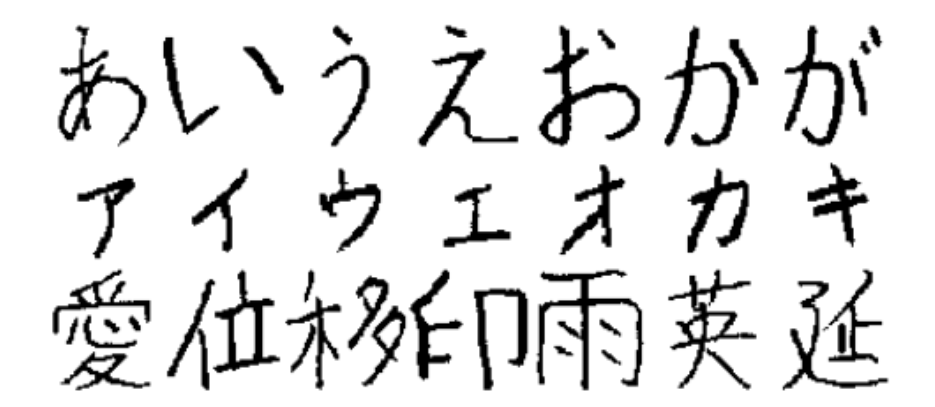
\includegraphics[width=\columnwidth]{kana}
	\caption{Extrahierte und invertierte Kana aus der ETL Character Database \cite[S.1]{RHC}.}
	\label{kana}
\end{figure}

Aus den umgewandelten Daten wurden zwei verschieden aufgebaute Datensätze erstellt. Der Erste ist am Paper von Charlie Tsai angelehnt und beinhaltet lediglich den ETL-1 Datensatz mit Katakana und den ETL-8 Datensatz mit Hiragana sowie Kanji \cite[S.3]{RHC}. Der Aufbau von diesem mit Unterteilungen in Hiragana, Katakana, Kanji und sonstiger Zeichen sowie das arithmetische Mittel der Datensätze pro Klasse und deren Standardabweichung lässt sich in der Tabelle \ref{data_tsai} erkennen.
\begin{table}[!htb]
	\caption{Aufbau des ersten Datensatz nach Charlie Tsai.}
	\label{data_tsai}
	\centering
	\begin{tabular}{|c|c|c|c|c|}
		\hline
		Alphabet & Klassen & Datensätze & Mean & Stddev\\
		\hline
		\hline
		Hiragana & 75 & 12.075 & 161 & 0\\
		\hline 
		Katakana & 48 & 71.959 & 1.499 & 342\\
		\hline
		Kanji & 881 & 141.841 & 161 & 0\\
		\hline
		Sonstige & 0 & 0 & 0 & 0\\
		\hline
		\hline
		Gesamt & 1.004 & 225.875 & 224 & 295\\
		\hline
	\end{tabular}
\end{table}

Wie klar zu sehen ist, sind Katakana im Gegensatz zu Kanji und Hiragana stark überrepräsentiert. Eine Nutzung von Klassengewichtungen, um die unterrepräsentierten Daten hervorzuheben, sollte sich daher als sinnvoll erweisen. Weiterhin stellt sich dies auch für die Katakana als möglicherweise sinnvoll heraus, da diese eine gewisse repräsentative Streuung aufweisen. Da der ETL-1 Datensatz ebenfalls Zeichen mit Beugungen (Dakuten und Handakuten) beinhaltet, besitzt der Datensatz deutlich mehr Klassen für Hiragana als Katakana, obwohl beide Alphabete sehr ähnlich aufgebaut sind. Mit einem Blick auf die originale Arbeit sind hier zwei Probleme zu erkennen. Zum einem hat sich die Anzahl der Datensätze seit dem originalen Paper um ca. 1000 erhöht \cite[S.3]{RHC}. Da hier kein Fehler beim Vorverarbeiten der Daten erkannt werden konnte, könnte es sich um ein Hinzufügen von Daten seitens der Verwalter der ETL Character Database handeln, was auch in einer Steigerung der Klassen der Kanji um drei resultiert. Weiterhin finden sich drei Katakanatypen weniger wieder. Dies hängt mit der Darstellung ausgestorbener Zeichen im ETL-1 Datensatz zusammen, welche die Buchstaben \textit{yi} zu \textit{i}, \textit{ye} zu \textit{e} und \textit{wu} zu \textit{u} werden lassen \cite{ETL}. Hier wurden im Gegensatz zur originalen Arbeit die daraus resultierenden Beispiele zu den passenden Vokalen umgeschrieben \cite[S.3]{RHC}. Eine gleichzeitge Erhöhung der Kanji und Verringerung der Katakana um drei, hat sich nach Prüfungen als zufällig herausgestellt. 

Mit diesem ersten Datensatz können einige praktische Probleme leider nicht gelöst werden. Soll Maschinelles Lernen zum Übersetzen von Sprache eingesetzt werden, so ist es nötig, die meisten Aspekte dieser Sprache zu berücksichtigen. Heutzutage hat sich das lateinische Alphabet in viele Aspekte der japanischen Sprache etabliert. Eine reine Erkennung japanischer Zeichen ist daher für praktische Anwendungen eher weniger sinnvoll. Auch Satzzeichen und Sonderzeichen wurden im originalen Datensatz nicht berücksichtigt, obwohl diese für ein späteres Verständnis ganzer Sätze essenziell sind. Zuletzt beinhaltet der Datensatz lediglich 881 der 2136 üblich genutzten Kanji \cite[S.3]{RHC}. Da die ETL Character Database noch weitere Datensätze beinhaltet, wurde sich entschieden, in einem weiteren Datensatz die gesamte Datenbank zu nutzen. Der Aufbau dieser Gesamtauswahl lässt sich in Tabelle \ref{data_total} erkennen.

\begin{table}[!htb]
	\caption{Aufbau des zweiten Datensatz als Gesamtauswahl der ETL Character Database.}
	\label{data_total}
	\centering
	\begin{tabular}{|c|c|c|c|c|}
		\hline
		Alphabet & Klassen & Datensätze & Mean & Stddev\\
		\hline
		\hline
		Hiragana & 77 & 67.335 & 874 & 437\\
		\hline 
		Katakana & 73 & 147.237 & 2.017 & 1.496\\
		\hline
		Kanji & 2.967 & 782.561 & 264 & 83\\
		\hline
		Sonstige & 74 & 175.308 & 2.369 & 1.013\\
		\hline
		\hline
		Gesamt & 3.191 & 1.172.441 & 367 & 507\\
		\hline
	\end{tabular}
\end{table}
Wie klar zu sehen ist, beinhaltet die gesamte ETL Character Database noch deutlich mehr Daten, welche für das Maschinelle Lernen genutzt werden können. So konnten die vorliegenden Kanji verdreifacht und die durchschnittlichen Datensätze pro Kanji nahezu verdoppelt werden. Weiterhin sind die Hiragana nicht mehr stark unterrepräsentiert und sonstige Zeichen wie aus dem lateinischen Alphabet oder Satzzeichen können erlernt werden. Eine größere Schwankung in der Durchschnittszahl der Datensätze sowie eine höhere Streuung dieser macht auch hier wieder eine Nutzung von Klassengewichtungen eine sinnvolle Ergänzung.

Eine beliebte Möglichkeit, das Overfitting von Modellen zu verringern sowie die Toleranz gegenüber Daten in der Praxis zu verbessern, ist die sogenannte Data Augmentation. Dabei können durch bestimmten Transformationen aus vorliegenden Daten neue generiert werden. Typische Vorgehensweisen bei Bildern sind dabei das skalieren, verschieben oder rotieren der Daten. Auch eine Spiegelung kann sich bei manchen Bilddaten als sinnvoll erweisen, jedoch würde dies die Bedeutung von Schriftzeichen zerstören. Werden Transformationen miteinander kombiniert, so kann die Anzahl der vorhandenen Daten um ein Vielfaches erhöht werden \cite[S.311]{MACHINE_LEARNING}. Im Code des Projekts können Skalierungen und Rotationen verwendet werden, um die Daten künstlich zu erhöhen. Dies geschieht über Transformationsmatrizen, welche mit der Bibliothek CV2 generiert und angewendet wurden. Eine Generation von 25 verschiedenen Transformationsmatrizen lässt sich in der Funktion im folgenden Listing \ref{listing1} erkennen.
\begin{lstlisting}[language=python,label=listing1,caption={Python-Code für die Generierung von Transformationsmatrizen}]
	
def create_transforms(
  format, 
  scale_values, 
  rot_values):
  
  if rot_values is None or len(rot_values) == 0:
    rot_values = [-20, -10, 0, 10, 20]
	
  if scale_values is None or len(scale_values) == 0:
    scale_values = [0.8, 0.9, 1.0, 1.1, 1.2]
	
  transform_matrices = []
  for rot_value in rot_values:
    for scale_value in scale_values:
      transform_matrix = cv2.getRotationMatrix2D(
        (format[0]/2, format[1]/2),
        rot_value, scale_value)
      transform_matrices.append(transform_matrix)

  return transform_matrices
\end{lstlisting}
Die Transformationsmatrizen würden bei der beispielhaften Anwendung auf dem Kanji \textit{zwei Stück} die Ausgabe in der Abbildung \ref{rot} erzeugen. Es ist klar die Skalierung zwischen den Größen und die Rotation zu erkennen, welche in einer Vergrößerung der Daten um den Faktor 25 resultieren würde.
\begin{figure}[!htb]
	% \centering
	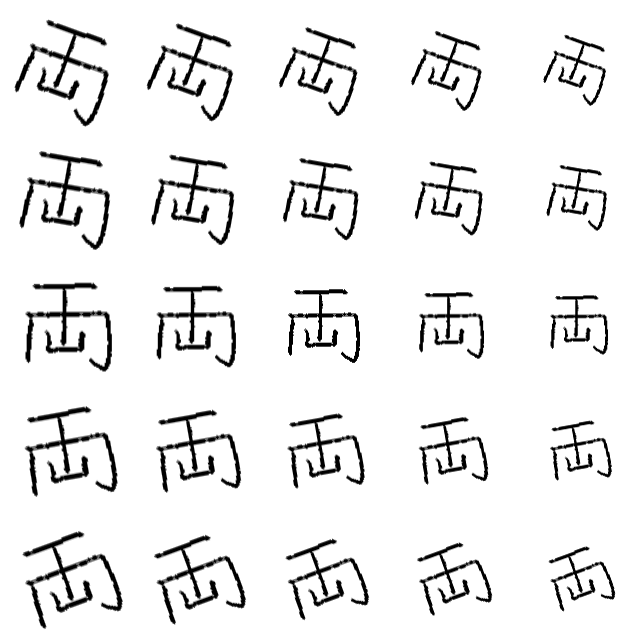
\includegraphics[width=\columnwidth]{rot_scale}
	\caption{Transformationen des Kanji \textit{zwei Stück}.}
	\label{rot}
\end{figure}
\section{Eingesetzte Modelle}
\begin{figure*}[!htb]
	\centering
	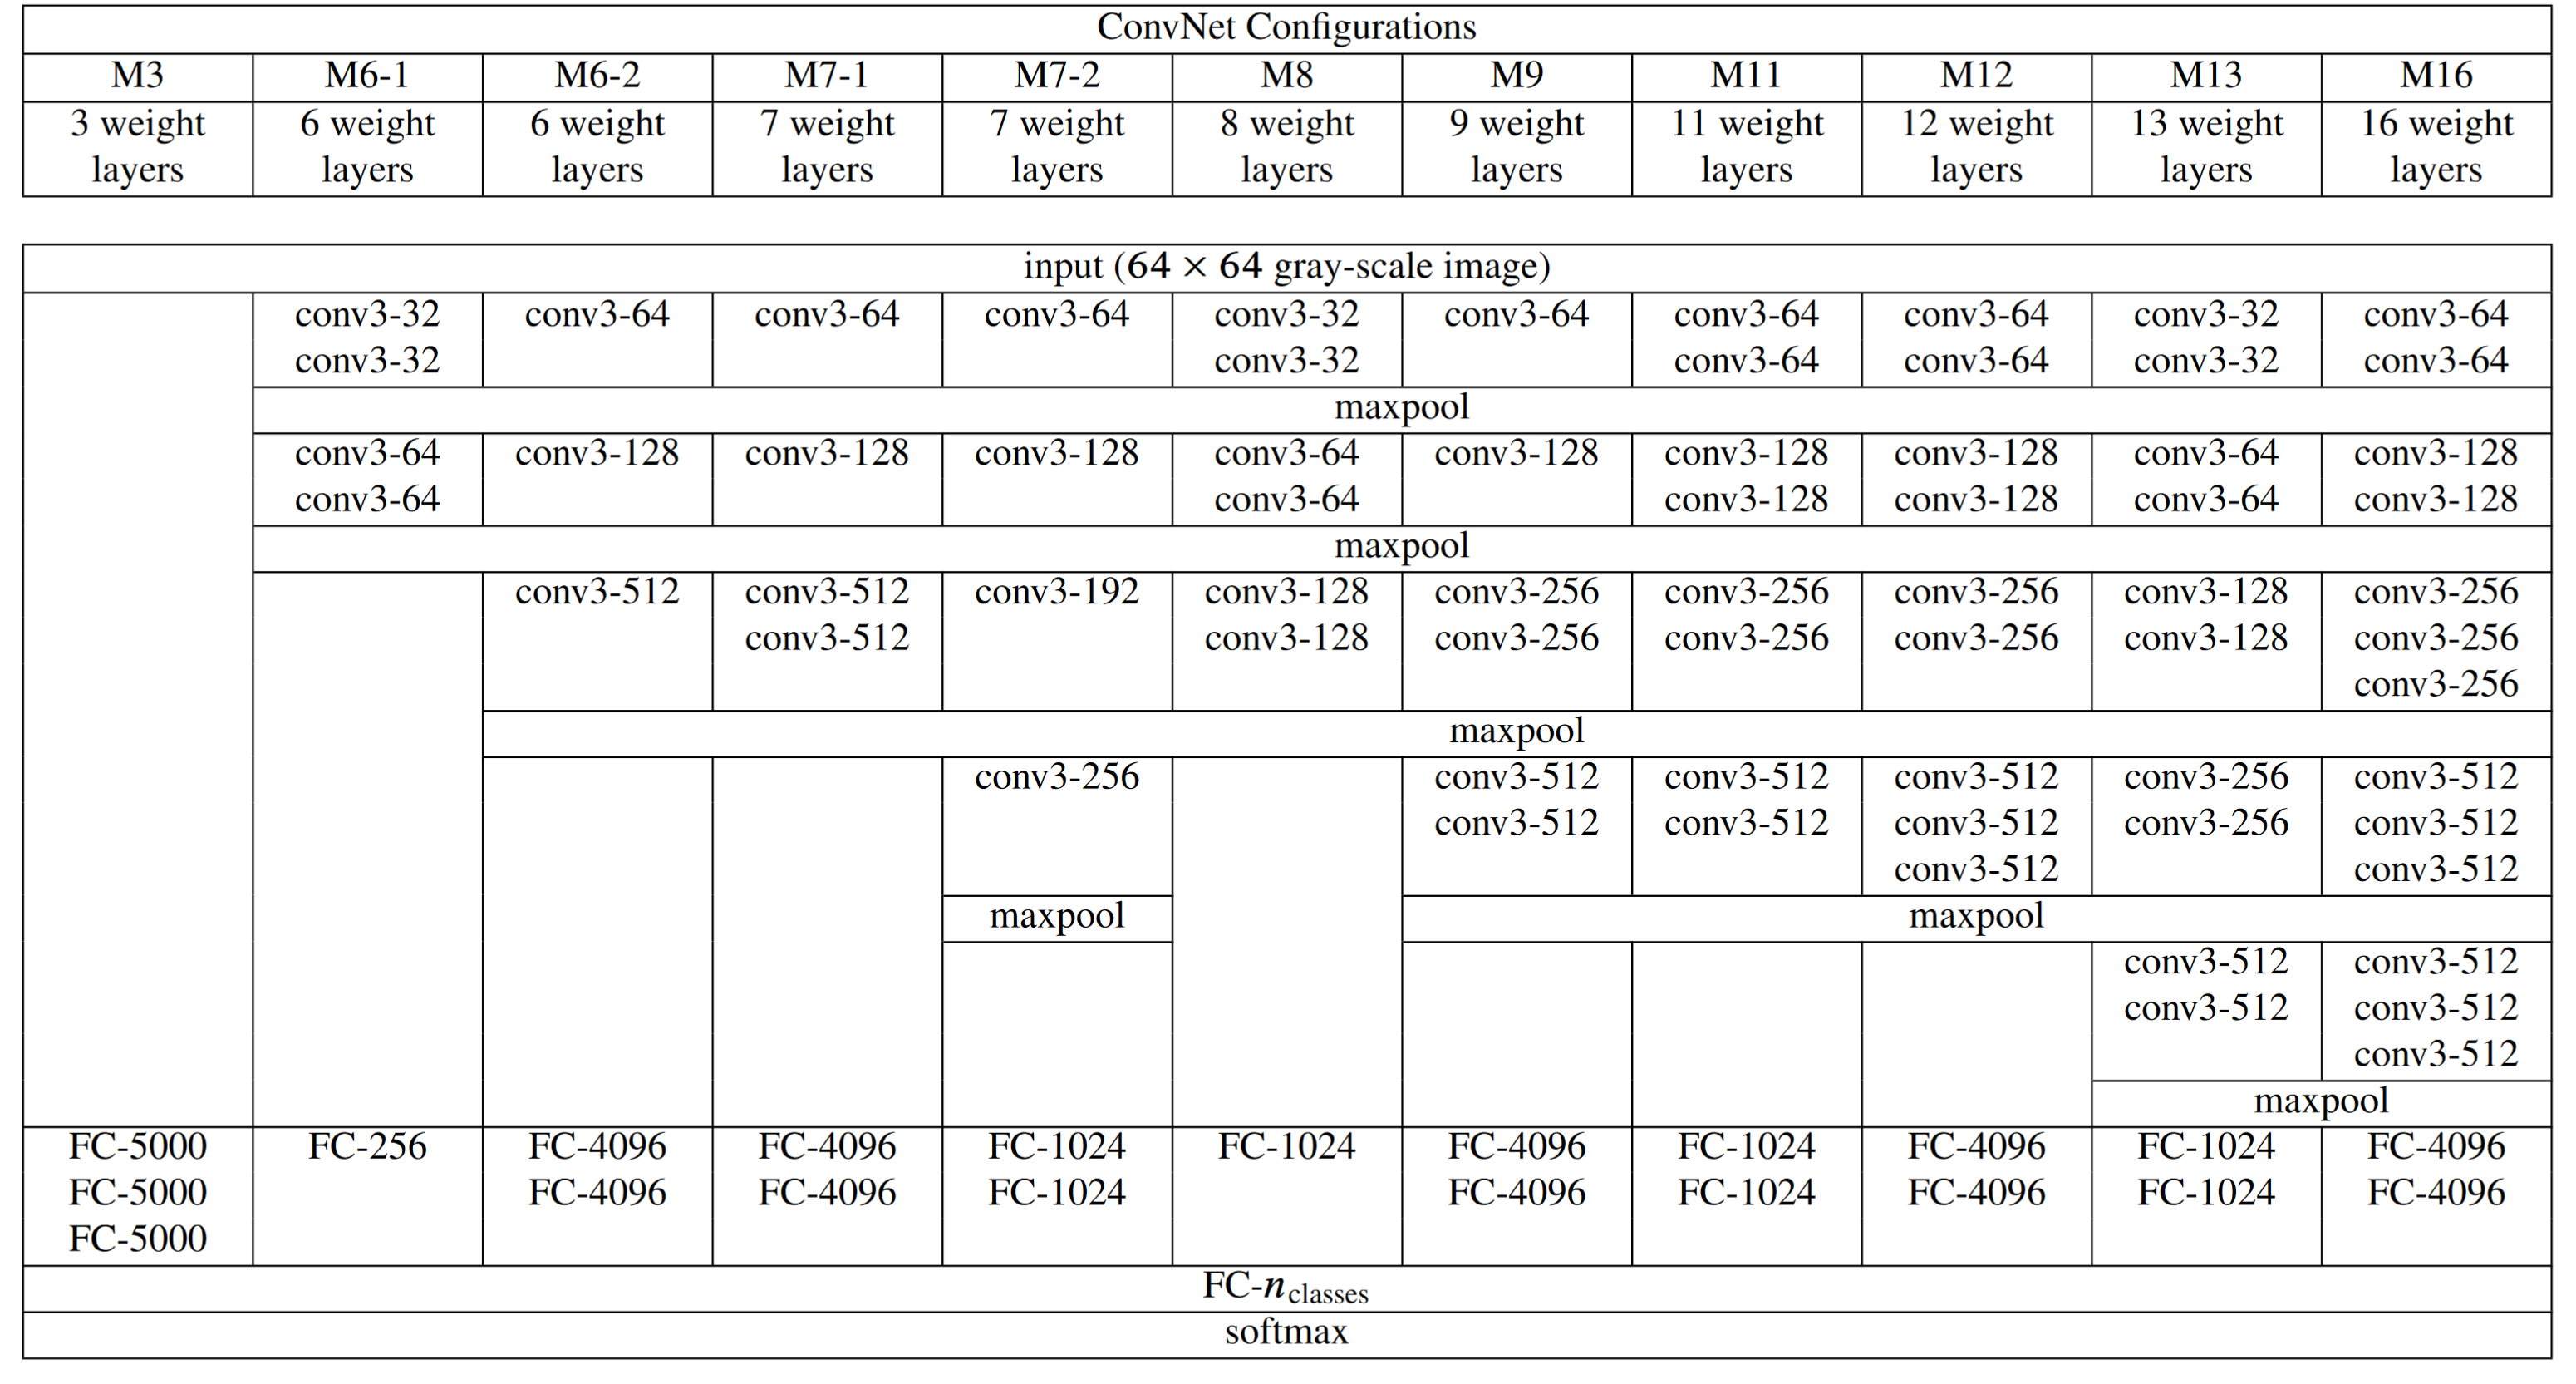
\includegraphics[width=2.1\columnwidth]{conv_net_architectures}
	\caption{Genutzte VGGNet Architekturen im Paper von Charlie Tsai \cite[S.3]{RHC}.}
	\label{vggnet}
\end{figure*}
Im Gegensatz zur originalen Arbeit von Charlie Tsai, wurde sich aufgrund der guten Ergebnisse bei einer gemeinsamen Erkennung aller Alphabete gegen die Nutzung von separaten Modellen für Kanji, Katakana und Hiragana entschieden. Dieses Vorgehen würde ein zusätzliche Modell zur Unterscheidung von Alphabeten benötigen und daher insgesamt vier Modelle nötig machen. Da die Ergebnisse für die Erkennung aller Alphabete laut Tsais Arbeit bereits bei sehr hohen 99,53\% in den Testdaten lagen, wurde sich gegen einen separaten Ansatz entschieden, um den Fokus auf die Erkennung aller Zeichen zu legen \cite[S.4-6]{RHC}. Aufgrund der teilweise hohen Streuung der Häufigkeiten von Datensätzen, wurden alle Ansätze mit Klassengewichtungen erprobt. Dies ist nötig, damit jedes Schriftzeichen unabhängig von der Häufigkeit in den Datensätzen in etwa gleich gut erkannt werden kann.

Während des Lernvorgangs wurden die Daten in 80\% Trainings- und jeweils 10\% Validierungs- und Testdaten geteilt. Alle Modelle wurden mit einem Adam-Optimizer trainiert, welcher auch in Tsais Arbeit genutzt wurde \cite[S.4]{RHC}. Die Startlernrate wurde dabei von Modell zu Modell verschieden angepasst. Es wurde weiterhin eine zerfallende Lernrate genutzt, welche alle 20 Epochen die Rate auf ein 0,9-Faches des ursprünglichen Wertes reduziert. Dies ist am Vorgehen von Tsai angelehnt \cite[S.4]{RHC}. Die Genauigkeit und der Verlust auf den Validierungsdaten wird mit jeder Epoche berechnet und dient als Maß des Fortschritt während des Trainings. Ein Training wird automatisch abgebrochen, falls nach 20 Epochen keine Verbesserung des Verlusts auftritt. Nach dem Training wird eine Übersicht generiert, welche den ungewichteten Durchschnitt des F1-Scores aller Klassen auf den Validierungsdaten als auch für einen späteren Vergleich zwischen den Modellen auf den Testdaten beinhaltet. Zusätzlich wird die Gesamtgenauigkeit ausgegeben.
\subsection{VGGNet}  %14.11 --- 
Der Architektur der VGGNet wurde in Simonyans und Zissermans Paper \textit{Very Deep Convolutional Networks for Large-Scale Image Recognition} entworfen und konnten 2015 state-of-the-art Genauigkeiten mit einem relativ einfachen sowie flexiblen Aufbau Konvolutionaler Neuronaler Netze erreichen \cite[S.1]{simonyan2015deep}. Sie arbeiten in den konvolutionalen Schichten typischerweise mit einem Wahrnehmungsfeld von 3 x 3 Elementen. Weiterhin nutzen sie ein 2 x 2 Max-Pooling mit einem Stride von 2. Das Max-Pooling tritt dabei nach einigen aber nicht jeder Schicht auf. Danach folgen zwei Fully Connected Schichten mit 4096 Neuronen und schließlich eine Fully-Connected Schicht mit Neuronen in Höhe der Anzahl der vorliegenden Klassen \cite[S.2]{simonyan2015deep}.

In Tsais Arbeit wurden 11 VGGNet artige Netze umgesetzt, welche in der Tabelle \ref{vggnet} von links nach rechts nach Netzgröße geordnet dargestellt werden. Diese weisen im Vergleich zum originalen VGGNet Paper einige Veränderungen in der Struktur auf. Zum einen liegen die Daten nur mit einem 64 x 64 Pixel Grauwertkanal vor \cite[S.3]{RHC}. Dadurch wird die Größe der Eingabedaten im Gegensatz zum originalen VGGNet Paper mit 224 x 224 Pixel RGB-Bildern sehr viel kleiner \cite[S.2]{simonyan2015deep}. Weiterhin wurde die Anzahl der Neuronen und Schichten im Fully-Connected Teil von Modell zu Modell angepasst \cite[S.3]{RHC}. Aufgrund der guten Ergebnisse der Klassifikation in der originalen Arbeit, wurde ein besonderer Fokus auf die Modelle M7-1, M7-2, M9 und M12 gesetzt \cite[S.5]{RHC}. Alle diese Netzen wurden nach Tsai mit einem Dropout versehen, welcher allerdings aufgrund Probleme bei höheren Raten auf 25\% verringert wurde und nur nach jeder Gruppe von Schichten platziert wurde \cite[S.2]{RHC}. Zusätzlich musste auf eine Batch-Normalisierung nach jeder Schicht verzichtet werden, da diese Probleme im Zusammenhang mit dem Dropout verursacht und die Ergebnisse stark verschlechtert hat \cite[S.4]{RHC}. Dank der direkten Unterstützung der Keras Applications API und der Möglichkeit des Transfer Learnings von \textit{imagenet} Gewichtungen, wurden zusätzlich die von Keras implementierten VGG16 und VGG19 Netze erprobt \cite{vgg_keras}.
\subsection{ResNet} %15.11
Die ResNet sind spezielle Architekturen Neuronaler Netze, welche mittels Restdarstellungen (Residual Representations) durch Abkürzungsverbindungen (Shortcut Connections) die Performanz tiefer Neuronaler Netze und im besonderen Konvolutionaler Netze verbessern sollen \cite[S.1-2]{resnet}. Dabei wird eine Ausgabe welche an einem bestimmten Punkt im Netzwerk ausgegeben wurde, an einem anderen Punkt identisch vor der Aktivierungsfunktion in die Ausgabe der tieferen Schicht eingerechnet \cite[S.4]{resnet}. Diese Funktionsweise lässt sich in der Abbildung \ref{res} am Beispiel zweier Schichten erkennen.
\begin{figure}[!htb]
	% \centering
	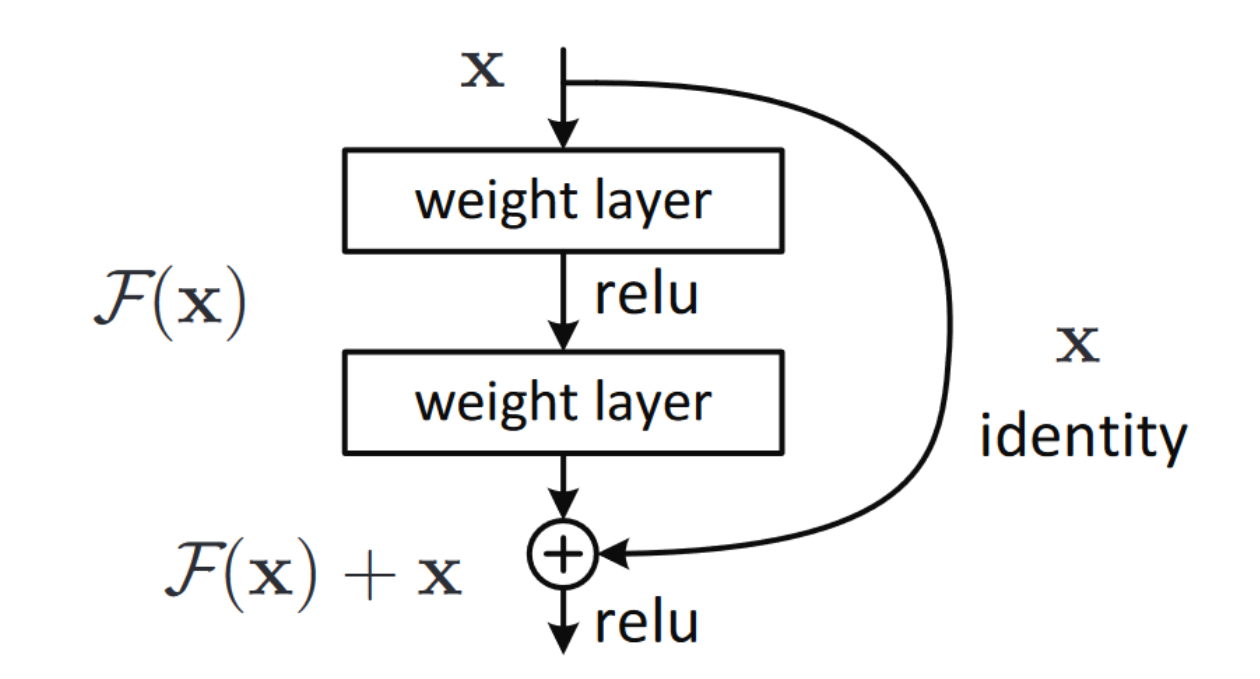
\includegraphics[width=\columnwidth]{residual}
	\caption{Beispiel einer Abkürzungsverbindung über zwei Schichten \cite[S.2]{resnet}.}
	\label{res}
\end{figure}


Ein solches Vorgehen soll den bei tiefen Neuronalen Netzen beobachteten Effekt des Zerfalls von Genauigkeiten bei einer zunehmenden Steigerung der Schichtenzahl bekämpfen \cite[S.1]{resnet}. Keras bietet in der Applications API für diese Netzarchitekturen sechs vordefinierte Modelle, welche 50, 101 bzw. 152 Schichten aufweisen \cite{resnet_keras}. Im besonderen wurde beim Trainieren ein Fokus auf die V2 Varianten dieser Modelle gesetzt, bei welchen es sich um eine Verbesserung des originalen Ansatz der ResNet handelt \cite{resnetv2}.
\subsection{Vision Transformer} %15.11
Vision Transformer wurden in vier verschiedenen Varianten erprobt, welche im Vision Transformer Paper dargestellt wurden. Es wurden dabei Modelle mit 12 (Base), 24 (Large) und 32 (Huge) Schichten vorgestellt, wobei die größte Variante aufgrund der wahrscheinlich nötigen Datenmenge nicht erprobt wurde. Alle Varianten der VIT mit ihren Parametern lassen sich in der Tabelle \ref{vit_sizes} erkennen. \cite[S.5]{VIT}. Die Base- und Large-Varianten wurden in der Version 16 und 32 erprobt, bei welcher es sich um die Dimensionen des Input Patchs handelt. Bei der Version 16 ist dieser 16x16 Pixel, während die Größe bei der Version 32 bei 32x32 Pixeln liegt \cite[S.5]{VIT}.
\begin{table}[!htb]
	\caption{Vordefinierte Varianten der Vision Transformer Modelle \cite[S.5]{VIT}.}
	\label{vit_sizes}
	\centering
	\begin{tabular}{|c|c|c|c|c|}
		\hline
		Modell & Schichten & Größe D & MLP Größe & Parameter\\
		\hline
		\hline
		Base & 12 & 768 & 3072 & 86M\\
		\hline
		Large & 24 & 1024 & 4096 & 307M\\
		\hline
		Huge & 32 & 1280 & 5120 & 632M\\
		\hline 
	\end{tabular}
\end{table}
In der Praxis wurden dieses über das Pythonpaket vit-keras, welches eine einfach und ähnlich zur Keras Applications API nutzbare Definition der ViT-Modelle ermöglicht. In diesem wurden alle nötigen Varianten implementiert und die Möglichkeit offen gehalten vorerlernte ImageNet-Gewichtungen zu laden \cite{git_vit}. Hier musste allerdings der Multilayer Perceptron Kopf der Vision Transformer selber definiert werden, da sonst Probleme mit der Ausgabe des Netzes auftraten. Zusätzlich mussten für die vorliegende Implementierung der Vision Transformer die Grauwertdaten in RGB Daten mit drei Kanälen umgewandelt werden. 
\section{Ergebnisse} %16.11
Die Ergebnisse aller trainierten Modelle, werden im Folgenden dargestellt. Hierbei sei zu beachten, dass aufgrund Zeitmangels einige Modelle nicht bis zum automatischen Abbruch des Trainings trainiert werden konnten. Diese wurden stattdessen nur 40 Epochen verbessert und sind über ein Asterisk am Modellnamen markiert. Beim Vergleich von Modellen wird bei den vorliegenden Ergebnisse der ungewichtete durchschnittliche F1-Score unserer Modelle mit der Genauigkeit des originalen Paper verglichen. Dies ergibt sich aufgrund unserer Nutzung von Klassengewichtungen, welche die Genauigkeit in der Tendenz schlechter werden lässt und den durchschnittlichen F1-Score zu einem besseren Vergleichspunkt macht. 

\subsection{VGGNet}

Mittels des Tsai Datensatz und der definierten VGG Netzen konnte sehr ähnliche Ergebnisse zum originalen Paper von Tsai erarbeitet werden. Es wurden für diesen Datensatz insgesamt sechs VGG Modelle trainiert, deren Ergebnisse in der Tabelle \ref{vgg_ergebnis_tsai} dargestellt werden.
\begin{table}[!htb]
	\caption{Genauigkeit und F1-Scores der VGGNet Modelle für den Tsai-Datensatz in Prozent.}
	\label{vgg_ergebnis_tsai}
	\centering
	\begin{tabular}{|c|c|c|c|c|}
		\hline
		Modell & Val-Acc & Test-Acc & Val-F1 & Test-F1\\
		\hline
		\hline
		M7-1 & 98,35 & 98,37 & 98,92 & 98,87\\
		\hline
		M7-2 & 98,04 & 98,25 & 98,95 & 98,95\\
		\hline
		M9 & 98,82 & 99,00 & 99,23 & 99,25\\
		\hline 
		M12 & \textbf{99,00} & \textbf{99,07} & \textbf{99,34} & \textbf{99,31}\\
		\hline 
		VGG16 & 97,97 & 98,21 & 98,64 & 98,63\\
		\hline 
		VGG19 & 97,68 & 97,58 & 98,32 & 98,10\\
		\hline 
	\end{tabular}
\end{table}

Das beste Modell M7-1 im originalen Paper konnte statt mit einer Genauigkeit von 99,39\% und 99,53\% nur einen durchschnittlichen F1-Score von 98,92\% und 98,87\% erreichen. Stattdessen konnte das Modell M12 mit 99,34\% und 99,31\% sehr vergleichbare Ergebnisse erlangen, während es in Tsais Paper schlechter abschnitt. Eine Abweichung von über einem halben Prozent im M7-1 ist bei Modellen, die schnell eine Genauigkeit von über 95\% erreichen enorm und eine zufällige Schwankung ist eher auszuschließen. Unterschiede beim Vorverarbeiten der Daten oder bei der Regularisierung, Techniken wie Dropout oder Batch-Normalisierung die einem Overfitting also einem Auswendiglernen der Eingabedaten entgegenwirken können \cite[S.27]{MACHINE_LEARNING}, in den Modellen, sind hierbei wahrscheinliche Hypothesen für die unterschiedlichen Ergebnisse. Unterschiede bei der Regularisierung könnte dabei ebenfalls eine Erklärung für das besseres abschneiden des M12 Modells sein. Die Modelle M7-2 und M9 liegen von ihren Ergebnissen zwischen M7-1 sowie M12 und weichen nicht viel von den des originalen Papers ab. Die zusätzlichen über Keras Applications API eingesetzten Modelle VGG16 und VGG19 schnitten leider durchweg schlechter als die vorher definierten Modelle ab. Da diese keine eingebaute Regularisierung bieten \cite{keras_vgg} und sie deutlich größer als die anderen Modelle ausfallen, könnten ein früheres Overfitting eine Erklärung für diese Ergebnisse sein.

Für den größeren kompletten Datensatz wurden die selben VGG Netze genutzt, wobei einige Modelle aufgrund hoher Rechenzeit nicht mehr zu Ende trainiert werden konnten. Die Ergebnisse dazu werden in der Tabelle \ref{vgg_ergebnis_full} dargestellt.
\begin{table}[!htb]
	\caption{Genauigkeit und F1-Scores der VGGNet Modelle für den kompletten Datensatz in Prozent.}
	\label{vgg_ergebnis_full}
	\centering
	\begin{tabular}{|c|c|c|c|c|}
		\hline
		Modell & Val-Acc & Test-Acc & Val-F1 & Test-F1\\
		\hline 
		\hline 
		M7-1 & 98,81 & 98,82 & 99,41 & 99,43\\
		\hline
		M7-2* & 96,60 & 96,57 & 98,36 & 98,38\\
		\hline
		M9 & 98,66 & 98,66 & 99,38 & 99,39\\
		\hline 
		M12 & \textbf{99,04} & \textbf{99,07} & \textbf{99,51} & \textbf{99,54}\\
		\hline 
		VGG16* & 97,84 & 97,92 & 98,47 & 98,57\\
		\hline 
		VGG19* & 98,00 & 98,08 & 98,61 & 98,70\\
		\hline 
	\end{tabular}
\end{table}

Erstaunlicherweise konnte dieser Datensatz trotz seiner Größe nahezu durchweg bessere Ergebnisse wie der Tsai-Datensatz liefern. Hier ist erneut das M12 Modell das Beste, welches mit 99,51\% und 99,54\% etwas bessere Ergebnisse im Vergleich zur originalen Arbeit liefert. Aber auch das M7-1 konnte die Ergebnisse verbessern und angleichen. Die anderen Modelle behalten das im vorherigen Abschnitt bezeichnete Verhalten bei, wobei die Ergebnisse leicht verbessert wurden.
\subsection{ResNet}

Die Ergebnisse der vorher genannten ResNet Modelle 50V2, 101V2 und 151V2 aus der Keras Applications API für den Tsai-Datensatz sind in der Tabelle \ref{resnet_ergebnis_tsai} dargestellt.
\begin{table}[!htb]
	\caption{Genauigkeit und F1-Scores der ResNet Modelle für den Tsai-Datensatz in Prozent.}
	\label{resnet_ergebnis_tsai}
	\centering
	\begin{tabular}{|c|c|c|c|c|}
		\hline
		Modell & Val-Acc & Test-Acc & Val-F1 & Test-F1\\
		\hline
		\hline
	 	50V2 & 98,42 & 98,47 & 98,83 & 98,78\\
		\hline
		101V2 & 98,55 & 98,57 & 98,87 & 98,80\\
		\hline
		151V2 & \textbf{98,62} & \textbf{98,74} & \textbf{98,95} & \textbf{98,96}\\
		\hline 
	\end{tabular}
\end{table} 
Das 151V2 konnte von diesen die besten Ergebnisse erreichen. Diese sind mit 98,95\% und 98,96\% in etwa vergleichbar mit den Ergebnissen des M7-1, aber sind damit leider geringer als die des M-12 Modells. Die anderen beiden Modelle erreichen leicht schlechtere Ergebnisse als das 151V2. 

Für die Resultate des kompletten Datensatz, welche in der Tabelle \ref{resnet_ergebnis_full} dargestellt werden, sieht dieses Bild etwas anders aus. Hier liefert das 101V2 Modell leicht bessere Ergebnisse wie das 151V2, obwohl beide Modelle die selbe (verkürzte) Zeit trainiert wurden. Es ist dabei allerdings durchaus möglich, dass bei einer Beendigung des Trainings eine deutliche Verbesserung des 151V2 stattfinden würde, was die Resultate zum Tsai-Datensatz spiegeln würde.
\begin{table}[!htb]
	\caption{Genauigkeit und F1-Scores der ResNet Modelle für den kompletten Datensatz in Prozent.}
	\label{resnet_ergebnis_full}
	\centering
	\begin{tabular}{|c|c|c|c|c|}
		\hline
		Modell & Val-Acc & Test-Acc & Val-F1 & Test-F1\\
		\hline
		\hline 
		50V2 & \textbf{98,66} & 98,65 & 99,09 & 99,07\\
		\hline
		101V2* & 98,63 & 98,65 & \textbf{99,05} & \textbf{99,11}\\
		\hline
		151V2* & 98,61 & \textbf{98,68} & 99,04 & 99,09\\
		\hline 
	\end{tabular}
\end{table}

Im Gegensatz zu den VGG-Netzen findet in der Keras Applications API in den ResNet Modellen Regularisierung per Batch-Normalisierung statt \cite{resnet_keras}. Zusätzlich nimmt die Genauigkeit beim Tsai-Datensatz mit komplexeren ResNet Modellen zu, was auch bei einer Vervollständigung des Trainings beim kompletten Datensatz der Fall seien könnte. Dies sind mögliche Indizien dafür, dass eine Verwendung noch größerer ResNet Modelle einen positiven Einfluss auf das Ergebnis haben könnte.
\subsection{Vision Transformer}
Für die Vision Transformer wurden vier verschiedene Modelle trainiert und die Ergebnisse für den Tsai-Datensatz sind in Tabelle \ref{vit_ergebnis_tsai} dargestellt. Diese konnten leider in keinster Weise die erwarteten Ergebnisse erreichen. Der beste Vision Transformer b32 konnte dabei 83,20\% und 83.58\% durchschnittlichen F1-Score erreichen und ist damit deutlich schlechter als jedes VGG oder ResNet Modell.
\begin{table}[!htb]
	\caption{Genauigkeit und F1-Scores der ViT Modelle für den Tsai-Datensatz in Prozent.}
	\label{vit_ergebnis_tsai}
	\centering
	\begin{tabular}{|c|c|c|c|c|}
		\hline
		Modell & Val-Acc & Test-Acc & Val-F1 & Test-F1\\
		\hline
		\hline
		b16* & 65,78 & 65,67 & 65,67 & 71,59\\
		\hline
		b32* & \textbf{74,76} & \textbf{75,63} & \textbf{83,20} & \textbf{83,68}\\
		\hline
		l16* & 69,07 & 69,10 & 74,52 & 74,83\\
		\hline
		l32* & 70,75 & 71,28 & 81,87 & 82,13\\
		\hline 
	\end{tabular}
\end{table}

Ähnlich sind die Ergebnisse für den kompletten Datensatz bei welchen der b32 Vision Transformer x\% und x\% erreichen konnte. Auf das Training der l32 und l16 Transformer mit dem kompletten Datensatz musste aufgrund zeitlicher Restriktionen verzichtet werden.
\begin{table}[!htb]
	\caption{Genauigkeit und F1-Scores der ViT Modelle für den kompletten Datensatz in Prozent.}
	\label{vit_ergebnis_full}
	\centering
	\begin{tabular}{|c|c|c|c|c|}
		\hline
		Modell & Val-Acc & Test-Acc & Val-F1 & Test-F1\\
		\hline
		\hline 
		b16* & 0 & 0 & 0 & 0\\
		\hline
		b32* & 0 & 0 & 0 & 0\\
		\hline 
	\end{tabular}
\end{table}

Für das schlechte Abschneiden der Vision Transformer in dieser Arbeit gibt es einigen Hypothesen. Zum einen benötigen Vision Transformer eine große Anzahl an Bildern, um mit CNNs vergleichbare Ergebnisse zu erreichen. Selbst der ImageNet Datensatz mit 14 Millionen Bildern \cite{IMAGENET} erreicht noch schlechtere Ergebnisse mit Vision Transformern als mit vergleichbaren CNNs \cite{JFT}. Die vorliegenden Datensätze für Kanji besitzen dagegen nur 225.000 und 1,2 Millionen Bilder. Eine weitere Möglichkeit für Probleme beim Training, könnte eine fehlende Eignung der genutzten ViT sein. Diese haben unabhängig der vorliegenden Grauwertdaten eine Eingabe von RGB-Daten verlangt, wodurch die Komplexität der Daten durch die Simulation von drei Eingabekanälen gestiegen seien könnte. Eine mögliche Nutzung anderer Bibliotheken für Vision Transformer, welche Grauwertdaten unterstützen und auf diese ausgelegt sind, könnten dieses Problem lösen. Die Nutzung von Huggingface, eine beliebte Community und Sammlung für Transformer \cite{huggingface}, und deren Python-API wäre ein möglicher nächster Schritt zur Verbesserung der Vorhandenen und dem Einsatz weiterer Transformer. Hier sollten auch Nachforschungen für spezielle Vision Transformer zur Texterkennung getroffen werden. 

\section{Fazit} %17.11
Alles in allem konnte das Projekt erfolgreich umgesetzt werden und die Ergebnisse der originalen Arbeit wurden nachvollzogen. Durch eine Simulation des Datensatz von Tsai, konnten sehr ähnliche Resultate erreicht werden, wodurch im Folgenden ein Einsätzen weiterer Modelle und eines Datensatz möglich war. Eine Nutzung neuer VGG, ResNet und Vision Transformer Modelle mit dem Datensatz, konnten leider die Ergebnisse nicht verbessern. Besonders die Vision Transformer haben sich dabei als problematisch herausgestellt. Trotzdem konnte durch die Erweiterung der genutzten Daten auf die gesamte ETL Character Database, die Klassifikation auf 3191 Schriftzeichen erweitert werden, während das beste VGG Modell für diesen Datensatz die Ergebnisse in der originalen Arbeit sogar minimal übertreffen konnte.
\section{Ausblick}
In zukünftigen Arbeiten ergeben sich zwei Wege des Vorgehens. Zum einen könnte vorhandene Modelle weiter verbessert und der Einsatz weiterer Techniken erprobt werden. Hierbei ist es denkbar die VGG16 und VGG19 mit Regularisierung oder größere ResNet zu erproben. Auch ein Einsatz von Vision Transformern mit Huggingface und eine Sichtung weiterer Modelle in der Huggingface Community, wären ein möglicher nächster Schritt. Der Einsatz der implementierten Techniken der Data Augmentation und die Nutzung der durch diese vergrößerten Datensätze wären ebenfalls ein wichtiges nächstes Vorgehen. Auf ein Training dieser musste leider aufgrund begrenzter Zeit verzichtet werden, da diese, aufgrund der enormen Steigerung der Daten, bereits mehr als einen Tag Rechenzeit pro Trainingsepoche in Anspruch genommen haben. Zusätzlich wäre eine Sichtung weiterer Datensätzen für Kanji zur Erweiterung der Datenbasis ein sinnvolles Vorgehen.

Ein weiterer Weg für zukünftige Arbeiten, wäre die Nutzung der erstellten Modelle für praktische Anwendungen. Da diese bereits sehr gute Ergebnisse liefern, wäre ein erster Test in einer praktischen Anwendung ein möglicher Schritt. Hierbei könnten die Modelle verwendet werden, um unbekannte Schriftzeichen analysieren und in einem Lexikon anzeigen zu lassen. Auch eine Live-Übersetzung japanischer Texte, ähnlich zur App von Google Übersetzer, wäre ein mögliches größeres Projekt, bei dem die trainierten Modelle zum Einlesen japanischer Zeichen verwendet werden können.
%%% Literaturverzeichnis
\bibliographystyle{IEEEtran}
\bibliography{seminar}

%% oder manuell
%\begin{thebibliography}{1}
%
%\bibitem{IEEEhowto:kopka}
%H.~Kopka and P.~W. Daly, \emph{A Guide to \LaTeX}, 3rd~ed.\hskip 1em plus
%  0.5em minus 0.4em\relax Harlow, England: Addison-Wesley, 1999.
%
%\end{thebibliography}

\end{document}